% Preamble
\documentclass{beamer}
\usepackage[spanish]{babel}

% Packages
\usepackage{amsmath}
\usepackage[utf8]{inputenc}
\usepackage[T1]{fontenc}
\usepackage{graphicx}
\usepackage{algorithmicx}
\usepackage{algpseudocode}
\usetheme[compress]{Berlin}
\setbeamertemplate{page number in head/foot}[framenumber]

\title[Autómatas Celulares]{Autómatas Celulares: Bandadas de Agentes Autopropulsados}
\subtitle{72.25 - Simulación de Sistemas}
\author[Flores Lucey, Llanos]{Alejo Flores Lucey\inst{1} \and Nehuén Gabriel Llanos\inst{2}}
\institute[Instituto Tecnológico de Buenos Aires]
{
    \inst{1}
    \href{mailto:afloreslucey@itba.edu.ar}{afloreslucey@itba.edu.ar}\\
    Legajo 62622
    \and
    \inst{2}
    \href{mailto:nllanos@itba.edu.ar}{nllanos@itba.edu.ar}\\
    Legajo 62511
}
\date{2024 1C | Grupo Nº3}

\pgfdeclareimage[height=0.5cm]{university-logo}{itba}
\logo{\pgfuseimage{university-logo}}

% If you wish to uncover everything in a step-wise fashion, uncomment
% the following command:

%\beamerdefaultoverlayspecification{<+->}


\begin{document}

    \begin{frame}
        \titlepage
    \end{frame}

    \begin{frame}{Outline}
        \tableofcontents
        % You might wish to add the option [pausesections]
    \end{frame}


% Since this a solution template for a generic talk, very little can
% be said about how it should be structured. However, the talk length
% of between 15min and 45min and the theme suggest that you stick to
% the following rules:

% - Exactly two or three sections (other than the summary).
% - At *most* three subsections per section.
% - Talk about 30s to 2min per frame. So there should be between about
%   15 and 30 frames, all told.

    \section{Introducción}

    \begin{frame}{Introducción}
        \begin{itemize}
            \item
            El objetivo es representar el comportamiento de un sistema de partículas autopropulsadas (Off Lattice)
            en un espacio bidimensional.
            \item
            La implementación del modelo permite simular el sistema de partículas.
            \item
            Se definen observables que caracterizan el comportamiento del sistema.
        \end{itemize}
    \end{frame}

%    \subsection[Short First Subsection Name]{First Subsection Name}
%
%    \begin{frame}{Make Titles Informative. Use Uppercase Letters.}{Subtitles are optional.}
%        % - A title should summarize the slide in an understandable fashion
%        %   for anyone how does not follow everything on the slide itself.
%
%        \begin{itemize}
%            \item
%            Use \texttt{itemize} a lot.
%            \item
%            Use very short sentences or short phrases.
%        \end{itemize}
%    \end{frame}
%    \begin{frame}{Ejemplo para este frame}
%
%        You can create overlays\dots
%        \begin{itemize}
%            \item using the \texttt{pause} command:
%            \begin{itemize}
%                \item
%                First item.
%                \pause
%                \item
%                Second item.
%            \end{itemize}
%            \item
%            using overlay specifications:
%            \begin{itemize}
%                \item<3->
%                First item.
%                \item<4->
%                Second item.
%            \end{itemize}
%            \item
%            using the general \texttt{uncover} command:
%            \begin{itemize}
%                \uncover<5->{\item
%                First item.}
%                \uncover<6->{\item
%                Second item.}
%            \end{itemize}
%        \end{itemize}
%    \end{frame}

    \subsection{Sistema Real}

    \begin{frame}{Sistema Real}
        \begin{itemize}
            \item
            El modelo Off Lattice busca analizar el movimiento de un conjunto de partículas y cómo se produce un efecto
            de agrupamiento cuando interactúan entre sí.
        \end{itemize}
        \begin{minipage}[t]{0.5\textwidth}
            \begin{itemize}
                \item
                Este fenómeno se observa en la naturaleza en:
                \begin{itemize}
                    \item Bandadas de aves.
                    \item Cardúmenes de peces.
                    \item Movimiento de bacterias.
                \end{itemize}
            \end{itemize}
        \end{minipage}
        \begin{minipage}[t]{0.45\textwidth}
            \begin{figure}[H]
                \centering
                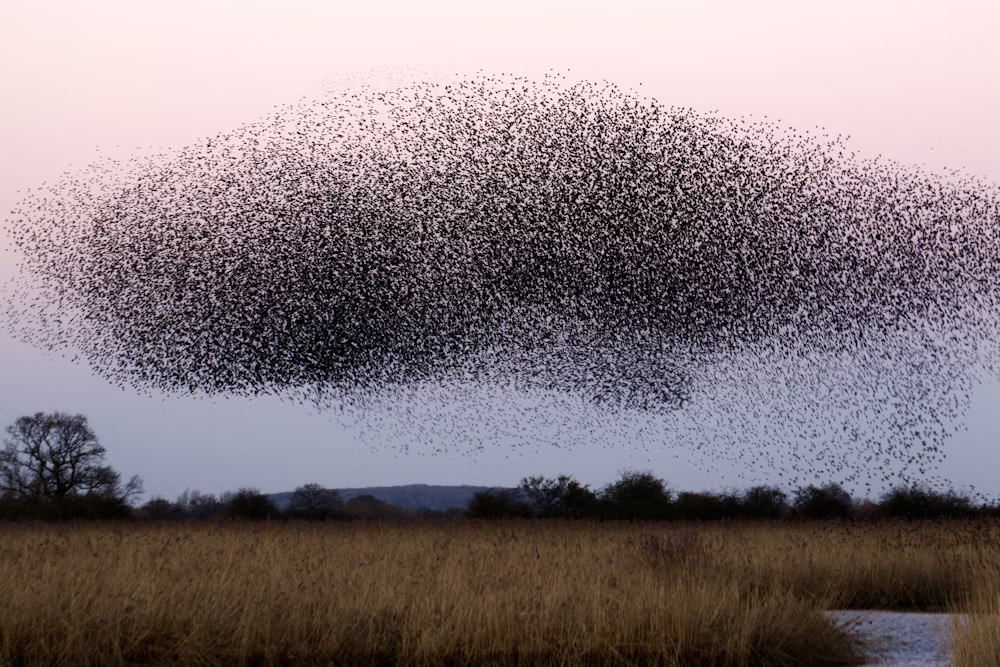
\includegraphics[width=\linewidth]{./bandadas_de_aves}
                \label{fig:bandadas_de_aves}
            \end{figure}
        \end{minipage}
    \end{frame}

    \subsection{Fundamentos}

    \begin{frame}{Fundamentos}
        \begin{itemize}
            \item El modelo de Bandadas de Agentes Autopropulsados se basa en dos ecuaciones principales:
                \begin{equation}
                    x_i(t+1) = x_i(t) + v_i(t) \Delta t\label{eq:equation1}
                \end{equation}
                \begin{equation}
                    \theta(t+1) = \langle \theta(t) \rangle_r+ \Delta \theta\label{eq:equation2}
                \end{equation}
            \item El $\langle \theta(t) \rangle_r$ es el promedio de los ángulos de las partículas vecinas:
                \begin{equation}
                    \langle \theta(t) \rangle_r = atan2(\langle sin(\theta(t)) \rangle_r, \langle cos(\theta(t)) \rangle_r)
                \end{equation}
        \end{itemize}
    \end{frame}

    \section{Implementación}

    \begin{frame}{Implementación}
        \begin{itemize}
            \item El modelo computacional se realizó en Java y cuenta con tres clases principales:
            \begin{itemize}
                \item \texttt{MovingParticle}: representa una partícula
                en el espacio.
                \item \texttt{OffLatticeAutomata}: representa el modelo de bandadas de agentes autopropulsados.
                \item \texttt{Main}: clase principal que ejecuta la simulación.
            \end{itemize}
        \end{itemize}
    \end{frame}

    \subsection{Arquitectura}
    \begin{frame}{Diagrama UML}
        \begin{figure}[htbp]
            \centering
            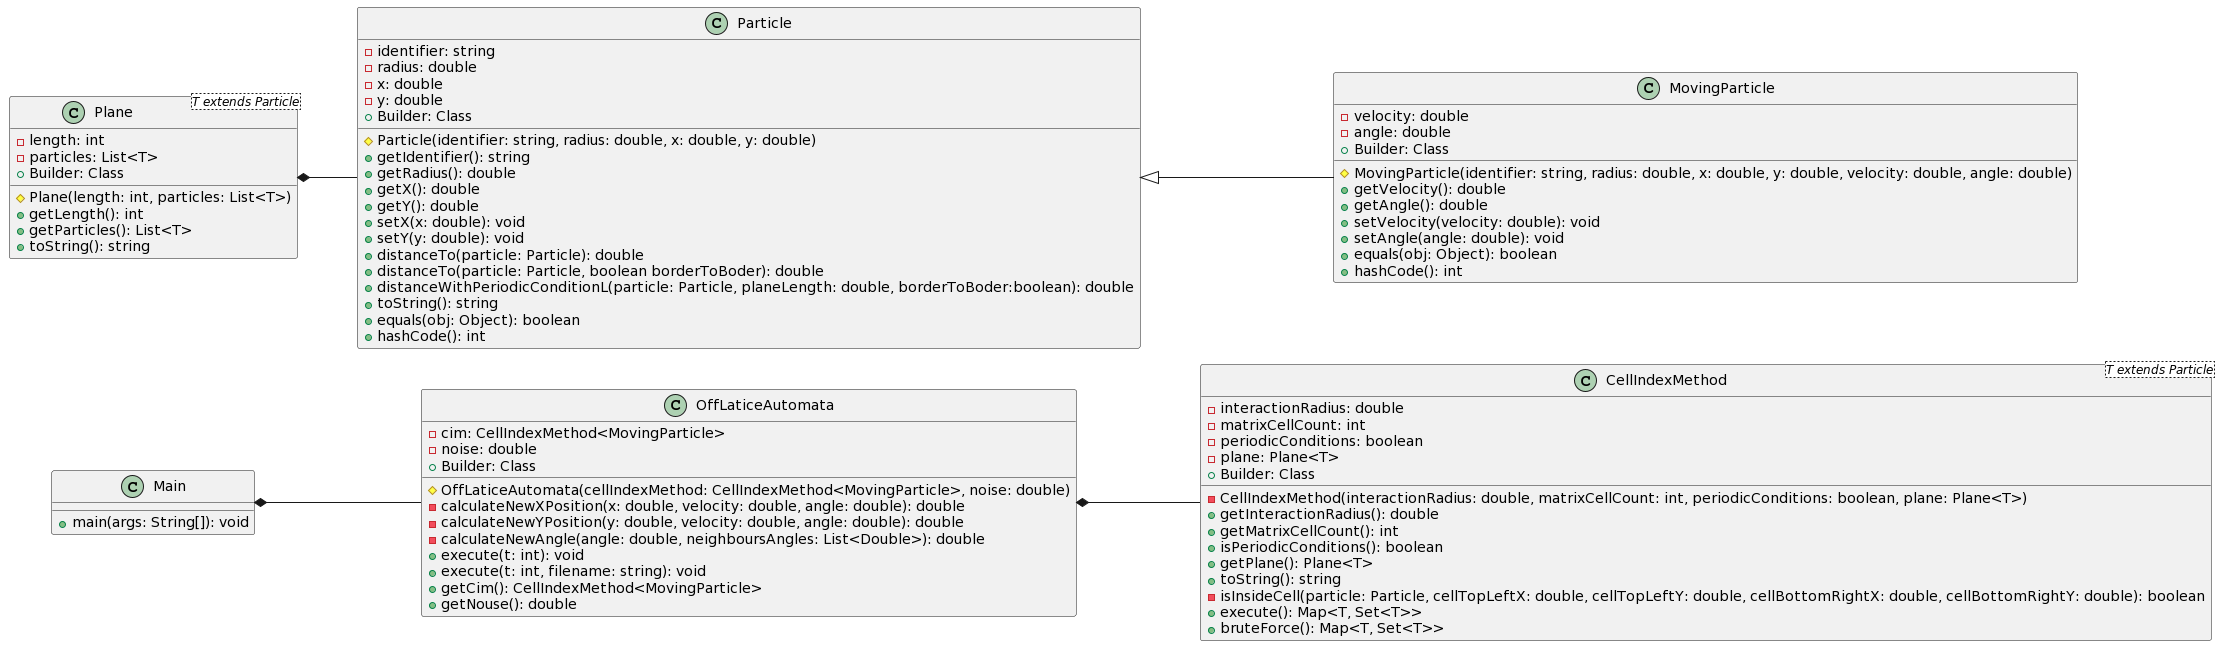
\includegraphics[width=\textwidth]{./architecture-landscape}
            \label{fig:architecture}
        \end{figure}
    \end{frame}

    \subsection{Algoritmo}
    \begin{frame}{Autómata Off Lattice}
        \begin{algorithmic}[1]
            \small
            \State Creación output de la simulación
            \While{$t < t_{max}$}
                \State CellIndexMethod()
                \State Obtención partículas vecinas de cada partícula en $t$
                \State Creación lista de objetos Partícula - ÁngulosVecinas en $t$
                \For{Par en lista de Partícula - ÁngulosVecinas}
                    \State Cálculo ángulo promedio de las partículas vecinas
                    \State Definición nuevo ángulo de la partícula en $t+1$
                    \State Actualización posición $x$ de la partícula en $t+1$
                    \State Actualización posición $y$ de la partícula en $t+1$
                    \State Escritura de información en output
                \EndFor
                \State Incremento del instante de tiempo $t$
            \EndWhile
        \end{algorithmic}
        \label{alg:algorithm}

    \end{frame}


    \section{Simulaciones}

    \begin{frame}{Simulaciones}
        Descripción del sistema particular que se va a simular y estudiar como
        geometría, rango de parámetros fijos y variables, inputs y outputs a estudiar. Ilustrar con un
        esquema el sistema particular que se va a simular.
        Además, se deben definir los observables que se calcularán a partir del output directo de la
        simulación (que presenta el estado del sistema para ciertos instantes de tiempo). Estas
        definiciones deben ser expresadas matemáticamente. Por ejemplo, si se va a promediar una cierta
        cantidad hay que explicitar cómo se promedia, que se va a estar sumando y sobre qué se estará
        dividiendo.
        Detallar el número de repeticiones y tiempos de las simulaciones realizadas.
    \end{frame}

    \section{Resultados}

    \subsection[Parámetro de Orden]{Parámetro de Orden}

    \begin{frame}{Animación}
        Estructurar la sección de resultados de la siguiente manera.
        2.4.1 Para cada input o parámetro a estudiar, primero mostrar una animación característica del
        sistema (pueden ser dos, con dos valores extremos del input para ver ejemplos de distintos
        comportamientos). La idea de esto es ilustrar la dinámica del sistema para situar el contexto de los
        resultados a mostrar.
    \end{frame}

    \begin{frame}{Observable en función del tiempo}
        2.4.2 Luego mostrar una figura del observable o métrica (que se calcula a partir de los outputs
        directos de la simulación) en función del tiempo. Explicar entonces cual será el escalar que
        caracteriza ese proceso (por ejemplo el promedio de la evolución temporal en el estado
        estacionario, la tasa de crecimiento, etc.). Solo mostrar evoluciones típicas, de valores extremos
        del rango de parámetros, para validar las definiciones de los observables. Las evoluciones en sí
        no son los resultados definitivos, por lo tanto no deben ser extenso lo que se muestre de las
        mismas solo para justificar el observable (escalar) que se calculará a partir de estas.
    \end{frame}

    \begin{frame}{Input vs observable}
        2.4.3 Después presentar la figura del input vs. observable, con promedio y barras de error o tablas
        con promedio y error.
    \end{frame}

    \subsection[Visitas PBC]{Visitas PBC: Tiempo en el que el nro. de visitas alcanza el 20\% de N}

    \begin{frame}{Animación}
        Estructurar la sección de resultados de la siguiente manera.
        2.4.1 Para cada input o parámetro a estudiar, primero mostrar una animación característica del
        sistema (pueden ser dos, con dos valores extremos del input para ver ejemplos de distintos
        comportamientos). La idea de esto es ilustrar la dinámica del sistema para situar el contexto de los
        resultados a mostrar.
    \end{frame}

    \begin{frame}{Observable en función del tiempo}
        2.4.2 Luego mostrar una figura del observable o métrica (que se calcula a partir de los outputs
        directos de la simulación) en función del tiempo. Explicar entonces cual será el escalar que
        caracteriza ese proceso (por ejemplo el promedio de la evolución temporal en el estado
        estacionario, la tasa de crecimiento, etc.). Solo mostrar evoluciones típicas, de valores extremos
        del rango de parámetros, para validar las definiciones de los observables. Las evoluciones en sí
        no son los resultados definitivos, por lo tanto no deben ser extenso lo que se muestre de las
        mismas solo para justificar el observable (escalar) que se calculará a partir de estas.
    \end{frame}

    \begin{frame}{Input vs observable}
        2.4.3 Después presentar la figura del input vs. observable, con promedio y barras de error o tablas
        con promedio y error.
    \end{frame}

    \subsection[Visitas OBC]{Visitas OBC: Nro. de visitas por unidad de tiempo}

    \begin{frame}{Animación}
        Estructurar la sección de resultados de la siguiente manera.
        2.4.1 Para cada input o parámetro a estudiar, primero mostrar una animación característica del
        sistema (pueden ser dos, con dos valores extremos del input para ver ejemplos de distintos
        comportamientos). La idea de esto es ilustrar la dinámica del sistema para situar el contexto de los
        resultados a mostrar.
    \end{frame}

    \begin{frame}{Observable en función del tiempo}
        2.4.2 Luego mostrar una figura del observable o métrica (que se calcula a partir de los outputs
        directos de la simulación) en función del tiempo. Explicar entonces cual será el escalar que
        caracteriza ese proceso (por ejemplo el promedio de la evolución temporal en el estado
        estacionario, la tasa de crecimiento, etc.). Solo mostrar evoluciones típicas, de valores extremos
        del rango de parámetros, para validar las definiciones de los observables. Las evoluciones en sí
        no son los resultados definitivos, por lo tanto no deben ser extenso lo que se muestre de las
        mismas solo para justificar el observable (escalar) que se calculará a partir de estas.
    \end{frame}

    \begin{frame}{Input vs observable}
        2.4.3 Después presentar la figura del input vs. observable, con promedio y barras de error o tablas
        con promedio y error.
    \end{frame}


    \section{Conclusiones}

    \begin{frame}{Conclusiones}
        (1 diapositiva): Basadas solo en los resultados mostrados, no son conclusiones
        resultados observados pero no mostrados en resultados, ni hipótesis de posibles explicaciones de
        lo observado que no hayan sido estudiadas explícitamente, cualquier hipótesis que
        potencialmente explique lo observado, debe ser probada explícitamente y mostrada en resultados,
        caso contrario no es válida como conclusión. Tampoco es una conclusión algo que haya quedado
        por hacer o algo que se haya hecho mal y se descartó.
    \end{frame}

%    \begin{frame}{Conclusiones}
%
%        % Keep the summary *very short*.
%        \begin{itemize}
%            \item
%            The \alert{first main message} of your talk in one or two lines.
%            \item
%            The \alert{second main message} of your talk in one or two lines.
%            \item
%            Perhaps a \alert{third message}, but not more than that.
%        \end{itemize}
%
%        % The following outlook is optional.
%        \vskip0pt plus.5fill
%        \begin{itemize}
%            \item
%            Outlook
%            \begin{itemize}
%                \item
%                Something you haven't solved.
%                \item
%                Something else you haven't solved.
%            \end{itemize}
%        \end{itemize}
%    \end{frame}


\end{document}
